Purpose of chapter, TODO

\section{Technology}
In this section, technologies used in triResolve that will be mentioned throughout this chapter are briefly described.

\subsection{Django}
Django is a Python web development framework \cite{holovaty_chapter_c1itd}. It implements a version of the MVC (Model-View-Controller) pattern, which decouples request routing, data access, and
presentation. Django's model layer allows the programmer to retrieve and modify entities in an SQL database through Python code, without writing SQL.

\subsection{MySQL}
MySQL is an open source relational database system \cite{what_wim}. It is used by TriOptima as the database backend for Django.

\subsection{Cassandra}
Cassandra is a column-oriented \textit{NoSQL} database \cite[p. 1-9]{mishra_2014_beginning_bacd}. It features dynamic schemas, meaning that columns can be added to a schema as needed, and that
the number of columns may vary from row to row. Cassandra is designed to have no single point of failure, and instead uses a number of nodes in a peer-to-peer structure. This design is
employed in order to ensure high availability, with data replicated across the nodes. It uses the query language CQL (Cassandra Query Language), which is similar to relational database SQL.

\section{Trade files and datasets}
As mentioned briefly in the background section, users of the triResolve service upload \textit{trade files}, which contain one or several datasets with
rows of trade data such as party id, counterparty id, trade id, notional, and so on. An example of a trade dataset (with some columns omitted) can be seen in figure
\ref{fig:data_set_example}.

\begin{figure}[ht]
\begin{tabular}{|c|c|c|p{3cm}|c|c|}%
  \hline
  \bfseries Party ID & \bfseries CP ID & \bfseries Trade ID & \bfseries Product class & \bfseries Trade curr & \bfseries Notional
  \csvreader[respect all,head to column names]{figures/EFET.csv}{PARTY_ID=\pid, CP_ID=\cpid, TRADE_ID=\tid, PRODUCT_CLASS=\pcls, TRADE_CURR=\tc, NOTIONAL=\notional}
  {\\\hline \pid & \cpid & \tid & \pcls & \tc & \notional}
  \\ \hline
\end{tabular}
  %\centering
\caption[Example of trade dataset]{A simplified example of a trade dataset uploaded by the users of triResolve.}
  \label{fig:data_set_example}
\end{figure}

\section{File formats}
Different customers may have different ways of formatting their datasets, with different names for headers, varying column orders, extra fields,
and special rules. In order to convert these into a common format that make it possible to use the files in the same contexts, a file format specifying
how the dataset in question should be processed is used. The format contains a set of \textit{filters} which should be applied to each row of the dataset.
The different filter configurations may affect how parallelizable the processing of dataset is. The result of this processing is called a \textit{verification result},
and consists of rows in a Cassandra schema.

\section{Filters}
All filters used to create a verification result are outlined below.

\subsection{Header detection}
There may be a number of lines in the dataset which do not contain the header (containing the column names). The header detection filter checks if a row is the header,
and if it is it saves the column names and corresponding indices for use in subsequent rows. If the row is not the header or the header has already been detected
(for example if another header row is encountered in the middle of the dataset), this filter terminates without any effect and the rest of the filters are applied.
This filter is included in all file formats.

\subsection{Mapping}
Maps a value from a column in the dataset to a specified output column in the verification result. This is usually specified for each of the columns in the input
dataset, and is therefore one of the most common filters. The mappings may have small extra tuning attached to them, such as specifying a date format or extracting only part of the
text using regex. One of these extra tunings is attached to the trade id column, and is called \textit{Make unique}. This tuning keeps track of all trade id:s that
have been encountered so far, and, if it finds a duplicate, adds a suffix to it in order to ensure that all trade id:s are unique.

\subsection{Dataset translation}
A dataset translation is similar to a mapping, but uses specified columns in an external dataset to map input columns to output columns.

\subsection{Dataset information}
Extracts information about the dataset, such as the name or owner.

\subsection{Tradefile information}
Similar to the dataset information filter, except that it extracts information about the trade file that contains the dataset.

\subsection{NullTranslationFilter}
In some datasets, other values than \code{NULL} are used to convey the absence of a value. This filter allows the user to specify which other values
should be interpreted as \code{NULL}.

\subsection{Relation currency}
If the currency that is supposed to be used in a relation (a party and a counterparty) is stored in the database and should be mapped to an output column, this
filter retrieves this information.

\subsection{Global variable}
A global variable filter writes a value to a variable that is accessed by subsequent filters on the same row, and by all filters on the rest of the rows in the data
set. A global variable can be written several times throughout the processing of a dataset.

\subsection{State variable}
A state variable is similar to a global variable, but is always written to before all other processing of the dataset begins.

\subsection{Temporary variable}
Similar to the other variables, except for the fact that it is only accessible during processing of the row where it was written. When the row has finished being
processed, the variable is cleared.

\subsection{Conditional block}
A conditional block works like the programming construct \code{if}. Performs a specified filter (which may also be a conditional block) only if a certain
condition is fulfilled. Most commonly, the condition takes the form \code{field = value}, but may also involve more complex expressions in the form of a
subset of Python.

\subsection{Logger}
A logger filter simply logs the specified output. Can for instance be used when a user wants to know whenever a conditional block has been entered.

\subsection{Skip row}
Ignores the current row when processing. Usually used in a conditional block.

\subsection{Stop processing}
Stops processing the dataset, ignoring all subsequent rows. Can be used as a subfilter in the Conditional block filter when the footer of the dataset
contains information that should not be interpreted as a trade.

\subsection{ThirdPartyAutoMapper}
When a customer has uploaded a trade file on behalf of another customer, this filter extracts the information needed to make sure that the data is loaded
for the correct customer.

\subsection{Set value}
Simply sets the value of the output column to the value that is entered.

\subsection{RegExp extract}
Extracts text from a column using regex, and writes matching groups to other columns.

\subsection{RegExp replace}
Replaces column text matching some regex with a specified value.

\section{Analyzing filters for parallelizability}
Since the filters specify what the processing program should do to each row in a dataset, "row by row" or possibly chunks of rows is a suitable
granularity when implementing the parallelization of the program. Consequently, the filters of a file format are the prime candidates
for parallelization analysis. The analysis made is similar to the methodology used to identify the span in the work-span model described in
section \ref{work-span}. When applying the model to the problem of analyzing filters, a task is the processing of one row. In order to find
the tasks that need to be completed before other tasks, the filters that result in state that is accessed by subsequent rows or otherwise
affect the total processing of the dataset need to be identified.

Looking through the filters, we can see that Dataset translation, NullTranslationFilter, Relation currency,
ThirdPartyAutomapper, Set value, RegExp extract, and RegExp replace only operate on the current dataset row, with no side effects.
This means that they produce no state changes that affect subsequent rows, which means that they do not affect the parallelizability of a dataset.

Additionally, Dataset information, Tradefile information, Temporary variable, Logger, and Skip row perform operations that either pull information from resources that
are available to all rows, or produce an effect that does not affect any other rows. The conditional filter only produces effects according to its subfilters (a set of
the filter already mentioned), and does not affect parallelization by itself.
\\\\
Hence, the filters that can affect the parallelization of a dataset are:
\begin{itemize}
  \item Mapping, since the trade id mapping may need to keep track of state that can be accessed in subsequent rows in order to make all id:s unique.
  \item Header detection, since all rows beneath the (first) header row depend on the column names for mappings and other values.
  \item Global variable, since the variable may be written and accessed by any subsequent rows. Each rewrite of the variable needs to happen before the next rewrite,
    in the original, sequential order if the verification result is to be correct.
  \item State variable, for the same reasons as Global variable.
  \item Stop processing, if one thread sees a conditional fulfilled and stops processing, it is possible for another thread to keep processing rows that are intended
    to be ignored.
\end{itemize}

\section{Program overview} %TODO: Skriv om loggning
The general flow of the original, sequential, dataset processing program is the following:
\\\\
The unprocessed dataset has the rows stored in a Cassandra database, and some metadata and methods stored in a Django object backed by a MySQL database.
The file format corresponding to the dataset is looked up, and all of the filters it contains are added to a pipeline that will process the dataset.
An empty verification result is then created in both Cassandra and MySQL, containing the row data and result metadata and metrics, respectively.
The metrics include processing time, number of trades, timestamp, and similar data. The rows in the dataset are then processed one by one,
applying all filters to each row. As soon as a row has finished processing, it is written to the verification result in Cassandra.
During this process, the row mappings used in the (common) Mapping filter are fetched from the MySQL database, resulting in some
I/O waiting time. To mitigate this, the mappings are cached in memory for faster access. After the processing has finished, the result metadata
and metrics are saved in the MySQL database.

\section{Implementation}

\subsection{Code inspection}
After an initial code and file format inspection, the following conclusions where made:
\begin{itemize}
  \item The header detection filter is effectively performed only once, as it is ignored for all rows after the one where the header was found.
  \item The filters Global variable and State variable make the processing of every row depend on the previous, as the writing of the variables may happen on each row.
  \item The process of making an ID unique could possibly be broken out to a post processing step.
  \item All file formats contain header detection, and many contain the make unique feature of the trade ID mapping.
  \item There are many file formats that do not have either Global variable, State variable or Stop processing among their filters.
\end{itemize}

The conclusions above indicate that header detection may be done before creating the parallel processes, sending this data to each process when they are created.
If the process of producing unique ID:s is then done as a post processing step, the following task DAGs illustrate how the dependencies when processing different
file formats appear. In figure \ref{fig:embarrassing_dag}, the task DAG for a file format without a Global variable or State variable filter is illustrated.
In figure \ref{fig:embarrassing_dag}, the task DAG for a file format containing a Global variable is illustrated. Since the span is equal to the work
in the file formats containing Global variables or State variables, parallelization of datasets with these formats will result in no speedup according to the
work-span model. File formats containing Stop processing become undecidable when parallelizing, since it is impossible to know if the result is correct if
any rows are processed in different processes (as rows that should not be included in the result may be included anyway).

\begin{figure}[ht]
  \centering
  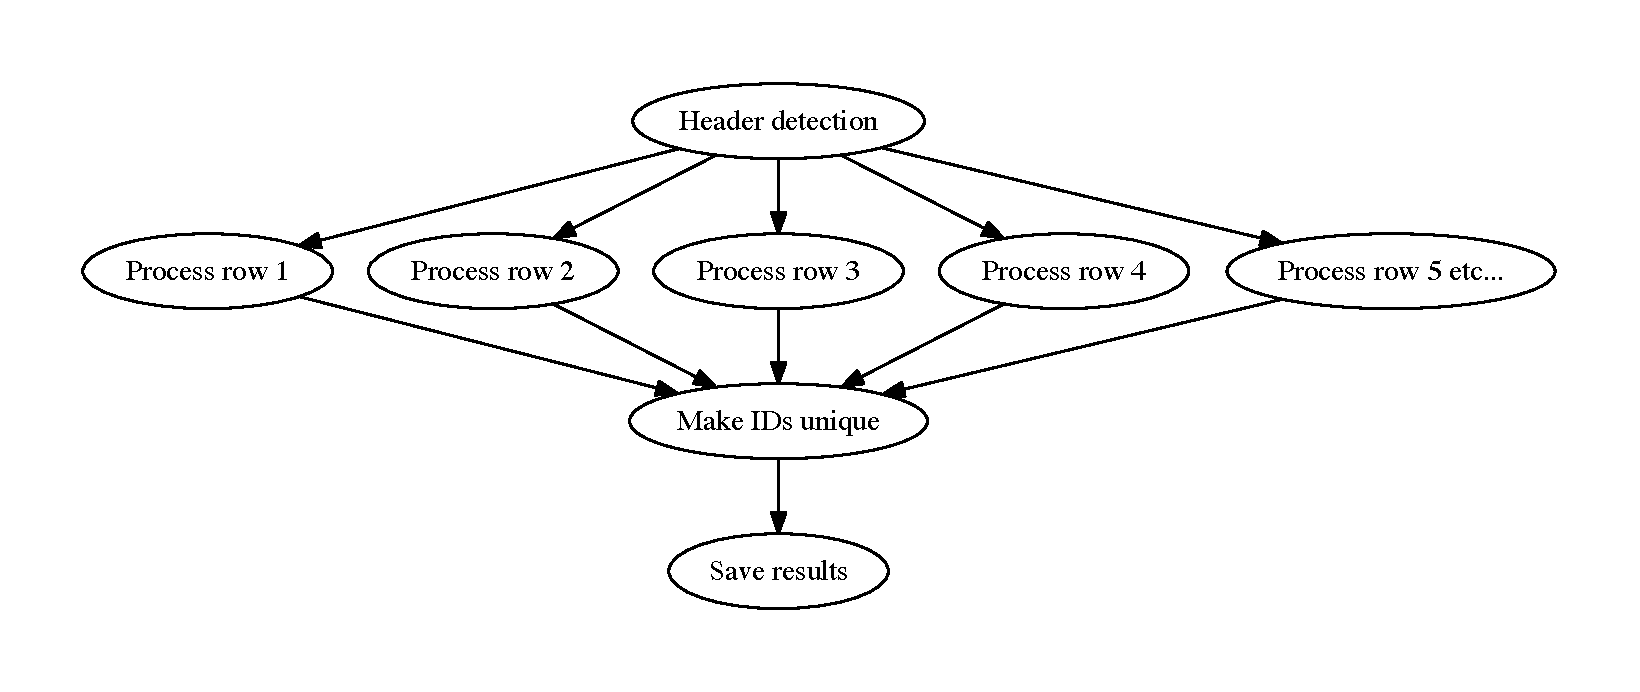
\includegraphics[width=120mm]{figures/embarrassing_file_format.pdf}
  \caption[Task DAG for a file format that does not contain global or state variables.]{An example of a task DAG for a file format that does not contain global variable or state variables. Header detections needs
  to be performed up front, and making trade IDs unique needs to be performed in a post processing step. The processing of each row does not depend on each other.}
  \label{fig:embarrassing_dag}
\end{figure}

\begin{figure}[ht]
  \centering
  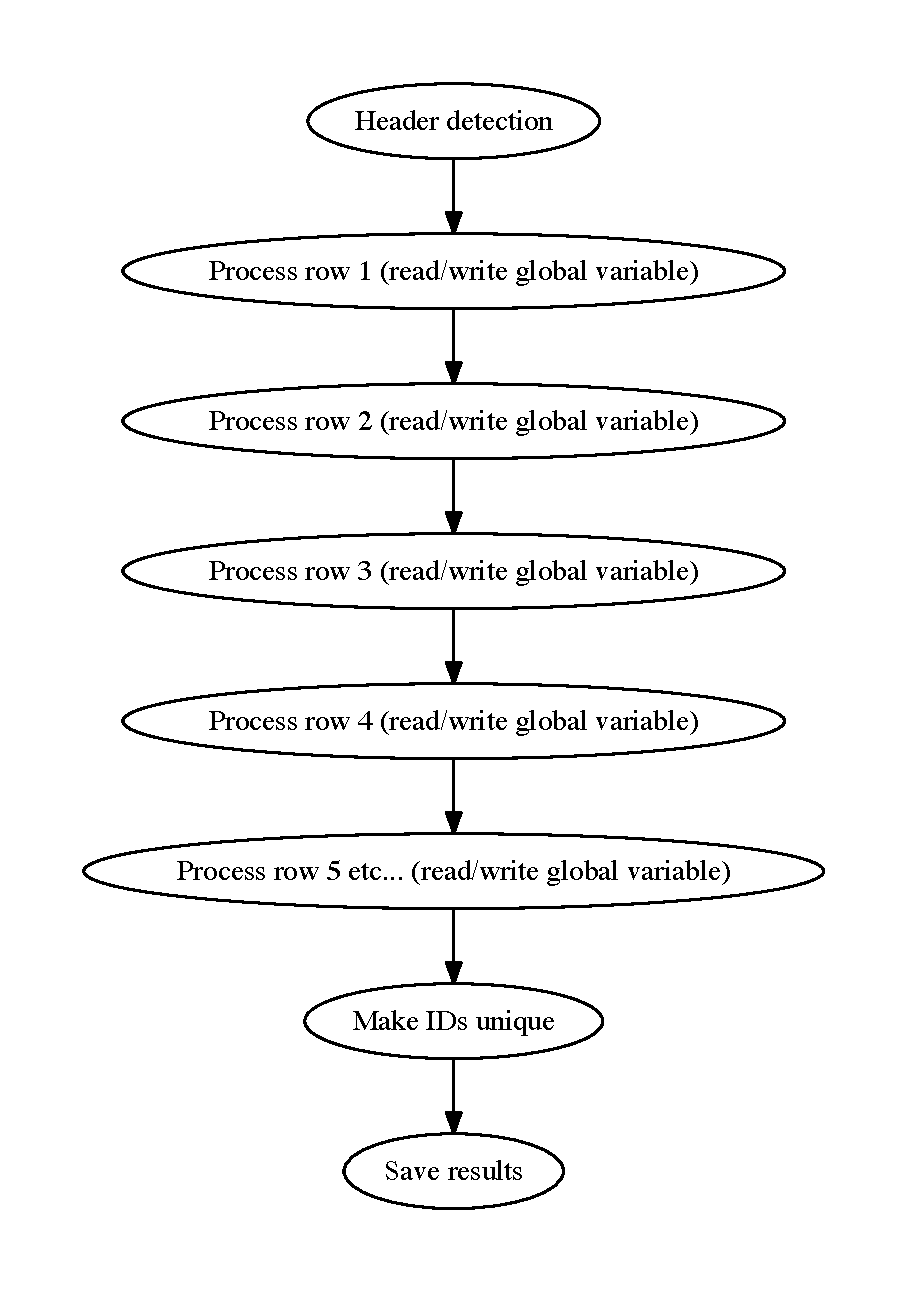
\includegraphics[width=120mm]{figures/global_variable_file_format.pdf}
  \caption[Task DAG for a file format that contains global or state variables.]{An example of a task DAG for a file format that contains global or state variables. Since each row may read and
  write the global (or state) variable, every task depends on the previous.}
  \label{fig:global_dag}
\end{figure}

\subsection{Parallelization}

\subsection{Sources of overhead}

\section{Evaluation}

